\documentclass[twoside]{book}

% Packages required by doxygen
\usepackage{fixltx2e}
\usepackage{calc}
\usepackage{doxygen}
\usepackage[export]{adjustbox} % also loads graphicx
\usepackage{graphicx}
\usepackage[utf8]{inputenc}
\usepackage{makeidx}
\usepackage{multicol}
\usepackage{multirow}
\PassOptionsToPackage{warn}{textcomp}
\usepackage{textcomp}
\usepackage[nointegrals]{wasysym}
\usepackage[table]{xcolor}

% Font selection
\usepackage[T1]{fontenc}
\usepackage[scaled=.90]{helvet}
\usepackage{courier}
\usepackage{amssymb}
\usepackage{sectsty}
\renewcommand{\familydefault}{\sfdefault}
\allsectionsfont{%
  \fontseries{bc}\selectfont%
  \color{darkgray}%
}
\renewcommand{\DoxyLabelFont}{%
  \fontseries{bc}\selectfont%
  \color{darkgray}%
}
\newcommand{\+}{\discretionary{\mbox{\scriptsize$\hookleftarrow$}}{}{}}

% Page & text layout
\usepackage{geometry}
\geometry{%
  a4paper,%
  top=2.5cm,%
  bottom=2.5cm,%
  left=2.5cm,%
  right=2.5cm%
}
\tolerance=750
\hfuzz=15pt
\hbadness=750
\setlength{\emergencystretch}{15pt}
\setlength{\parindent}{0cm}
\setlength{\parskip}{3ex plus 2ex minus 2ex}
\makeatletter
\renewcommand{\paragraph}{%
  \@startsection{paragraph}{4}{0ex}{-1.0ex}{1.0ex}{%
    \normalfont\normalsize\bfseries\SS@parafont%
  }%
}
\renewcommand{\subparagraph}{%
  \@startsection{subparagraph}{5}{0ex}{-1.0ex}{1.0ex}{%
    \normalfont\normalsize\bfseries\SS@subparafont%
  }%
}
\makeatother

% Headers & footers
\usepackage{fancyhdr}
\pagestyle{fancyplain}
\fancyhead[LE]{\fancyplain{}{\bfseries\thepage}}
\fancyhead[CE]{\fancyplain{}{}}
\fancyhead[RE]{\fancyplain{}{\bfseries\leftmark}}
\fancyhead[LO]{\fancyplain{}{\bfseries\rightmark}}
\fancyhead[CO]{\fancyplain{}{}}
\fancyhead[RO]{\fancyplain{}{\bfseries\thepage}}
\fancyfoot[LE]{\fancyplain{}{}}
\fancyfoot[CE]{\fancyplain{}{}}
\fancyfoot[RE]{\fancyplain{}{\bfseries\scriptsize Generated by Doxygen }}
\fancyfoot[LO]{\fancyplain{}{\bfseries\scriptsize Generated by Doxygen }}
\fancyfoot[CO]{\fancyplain{}{}}
\fancyfoot[RO]{\fancyplain{}{}}
\renewcommand{\footrulewidth}{0.4pt}
\renewcommand{\chaptermark}[1]{%
  \markboth{#1}{}%
}
\renewcommand{\sectionmark}[1]{%
  \markright{\thesection\ #1}%
}

% Indices & bibliography
\usepackage{natbib}
\usepackage[titles]{tocloft}
\setcounter{tocdepth}{3}
\setcounter{secnumdepth}{5}
\makeindex

% Hyperlinks (required, but should be loaded last)
\usepackage{ifpdf}
\ifpdf
  \usepackage[pdftex,pagebackref=true]{hyperref}
\else
  \usepackage[ps2pdf,pagebackref=true]{hyperref}
\fi
\hypersetup{%
  colorlinks=true,%
  linkcolor=blue,%
  citecolor=blue,%
  unicode%
}

% Custom commands
\newcommand{\clearemptydoublepage}{%
  \newpage{\pagestyle{empty}\cleardoublepage}%
}

\usepackage{caption}
\captionsetup{labelsep=space,justification=centering,font={bf},singlelinecheck=off,skip=4pt,position=top}

%===== C O N T E N T S =====

\begin{document}

% Titlepage & ToC
\hypersetup{pageanchor=false,
             bookmarksnumbered=true,
             pdfencoding=unicode
            }
\pagenumbering{alph}
\begin{titlepage}
\vspace*{7cm}
\begin{center}%
{\Large My Project }\\
\vspace*{1cm}
{\large Generated by Doxygen 1.8.13}\\
\end{center}
\end{titlepage}
\clearemptydoublepage
\pagenumbering{roman}
\tableofcontents
\clearemptydoublepage
\pagenumbering{arabic}
\hypersetup{pageanchor=true}

%--- Begin generated contents ---
\chapter{File Index}
\section{File List}
Here is a list of all files with brief descriptions\+:\begin{DoxyCompactList}
\item\contentsline{section}{src/\hyperlink{shm__client2_8c}{shm\+\_\+client2.\+c} }{\pageref{shm__client2_8c}}{}
\item\contentsline{section}{src/\hyperlink{shm__server2_8c}{shm\+\_\+server2.\+c} }{\pageref{shm__server2_8c}}{}
\end{DoxyCompactList}

\chapter{File Documentation}
\hypertarget{basic_8h}{}\section{include/basic.h File Reference}
\label{basic_8h}\index{include/basic.\+h@{include/basic.\+h}}


this header file contains the addition and substraction functions.  


This graph shows which files directly or indirectly include this file\+:\nopagebreak
\begin{figure}[H]
\begin{center}
\leavevmode
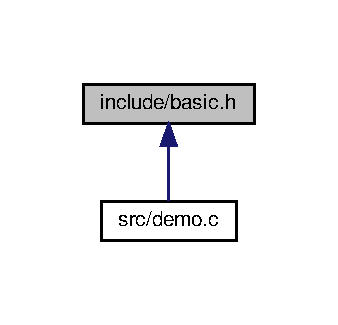
\includegraphics[width=162pt]{basic_8h__dep__incl}
\end{center}
\end{figure}
\subsection*{Functions}
\begin{DoxyCompactItemize}
\item 
int \hyperlink{basic_8h_ae9e80f72ea764075aace5d65cebc1ced}{add} (int, int)
\item 
int \hyperlink{basic_8h_ac296c54e8c35b1fb34f36f7b11c26ea3}{sub} (int, int)
\end{DoxyCompactItemize}


\subsection{Detailed Description}
this header file contains the addition and substraction functions. 

\begin{DoxyAuthor}{Author}
Rajat Bhagat
\end{DoxyAuthor}
\begin{DoxyDate}{Date}
08/26/2019 
\end{DoxyDate}


\subsection{Function Documentation}
\mbox{\Hypertarget{basic_8h_ae9e80f72ea764075aace5d65cebc1ced}\label{basic_8h_ae9e80f72ea764075aace5d65cebc1ced}} 
\index{basic.\+h@{basic.\+h}!add@{add}}
\index{add@{add}!basic.\+h@{basic.\+h}}
\subsubsection{\texorpdfstring{add()}{add()}}
{\footnotesize\ttfamily int add (\begin{DoxyParamCaption}\item[{int}]{a,  }\item[{int}]{b }\end{DoxyParamCaption})}

This function will add two numbers 
\begin{DoxyParams}{Parameters}
{\em a} & first argument \\
\hline
{\em b} & second argument \\
\hline
\end{DoxyParams}
\begin{DoxyReturn}{Returns}
returns sum
\end{DoxyReturn}
This function will add two numbers 
\begin{DoxyParams}{Parameters}
{\em a} & first argument \\
\hline
{\em b} & second argument \\
\hline
\end{DoxyParams}
\begin{DoxyReturn}{Returns}
returning the sum 
\end{DoxyReturn}
\mbox{\Hypertarget{basic_8h_ac296c54e8c35b1fb34f36f7b11c26ea3}\label{basic_8h_ac296c54e8c35b1fb34f36f7b11c26ea3}} 
\index{basic.\+h@{basic.\+h}!sub@{sub}}
\index{sub@{sub}!basic.\+h@{basic.\+h}}
\subsubsection{\texorpdfstring{sub()}{sub()}}
{\footnotesize\ttfamily int sub (\begin{DoxyParamCaption}\item[{int}]{a,  }\item[{int}]{b }\end{DoxyParamCaption})}

This function will sutract two numbers 
\begin{DoxyParams}{Parameters}
{\em a} & first argument \\
\hline
{\em b} & second argument \\
\hline
\end{DoxyParams}
\begin{DoxyReturn}{Returns}
returns difference 
\end{DoxyReturn}

\hypertarget{add_8c}{}\section{src/add/add.c File Reference}
\label{add_8c}\index{src/add/add.\+c@{src/add/add.\+c}}
\subsection*{Functions}
\begin{DoxyCompactItemize}
\item 
int \hyperlink{add_8c_aa99823a0fc8313c9c32541ce768fb801}{add} (int \hyperlink{stack_8c_ac387c78c380088dd0d9442c503960139}{a}, int b)
\end{DoxyCompactItemize}


\subsection{Function Documentation}
\mbox{\Hypertarget{add_8c_aa99823a0fc8313c9c32541ce768fb801}\label{add_8c_aa99823a0fc8313c9c32541ce768fb801}} 
\index{add.\+c@{add.\+c}!add@{add}}
\index{add@{add}!add.\+c@{add.\+c}}
\subsubsection{\texorpdfstring{add()}{add()}}
{\footnotesize\ttfamily int add (\begin{DoxyParamCaption}\item[{int}]{a,  }\item[{int}]{b }\end{DoxyParamCaption})}

This function will add two numbers 
\begin{DoxyParams}{Parameters}
{\em a} & first argument \\
\hline
{\em b} & second argument \\
\hline
\end{DoxyParams}
\begin{DoxyReturn}{Returns}
returning the sum 
\end{DoxyReturn}

\hypertarget{demo_8c}{}\section{src/demo.c File Reference}
\label{demo_8c}\index{src/demo.\+c@{src/demo.\+c}}
{\ttfamily \#include \char`\"{}basic.\+h\char`\"{}}\newline
{\ttfamily \#include $<$stdio.\+h$>$}\newline
Include dependency graph for demo.\+c\+:\nopagebreak
\begin{figure}[H]
\begin{center}
\leavevmode
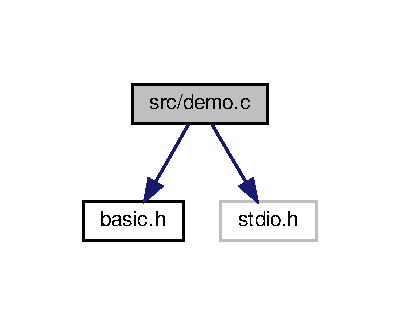
\includegraphics[width=192pt]{demo_8c__incl}
\end{center}
\end{figure}
\subsection*{Functions}
\begin{DoxyCompactItemize}
\item 
int \hyperlink{demo_8c_ae66f6b31b5ad750f1fe042a706a4e3d4}{main} ()
\end{DoxyCompactItemize}


\subsection{Function Documentation}
\mbox{\Hypertarget{demo_8c_ae66f6b31b5ad750f1fe042a706a4e3d4}\label{demo_8c_ae66f6b31b5ad750f1fe042a706a4e3d4}} 
\index{demo.\+c@{demo.\+c}!main@{main}}
\index{main@{main}!demo.\+c@{demo.\+c}}
\subsubsection{\texorpdfstring{main()}{main()}}
{\footnotesize\ttfamily int main (\begin{DoxyParamCaption}{ }\end{DoxyParamCaption})}

The function will demonstrate addition and substraction functions \begin{DoxyReturn}{Returns}
return type is int. 
\end{DoxyReturn}

\hypertarget{stack_8c}{}\section{src/stack.c File Reference}
\label{stack_8c}\index{src/stack.\+c@{src/stack.\+c}}
{\ttfamily \#include $<$stdio.\+h$>$}\newline
{\ttfamily \#include $<$stdlib.\+h$>$}\newline
Include dependency graph for stack.\+c\+:\nopagebreak
\begin{figure}[H]
\begin{center}
\leavevmode
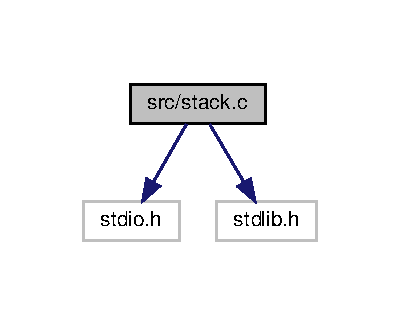
\includegraphics[width=192pt]{stack_8c__incl}
\end{center}
\end{figure}
\subsection*{Functions}
\begin{DoxyCompactItemize}
\item 
void \hyperlink{stack_8c_a614f20f3cfc81c55ede27b7b7cb66de9}{push} ()
\item 
int \hyperlink{stack_8c_a163177f1a0b7d847bc3241809dafc097}{pop} ()
\item 
void \hyperlink{stack_8c_a1e5b20fed15743656bb6d2e6a6ea6269}{display} ()
\item 
int \hyperlink{stack_8c_ae66f6b31b5ad750f1fe042a706a4e3d4}{main} ()
\end{DoxyCompactItemize}
\subsection*{Variables}
\begin{DoxyCompactItemize}
\item 
int \hyperlink{stack_8c_af93f4f37fc2ad9c37af4a715423b110c}{top} =-\/1
\begin{DoxyCompactList}\small\item\em initialised as empty stack \end{DoxyCompactList}\item 
int \hyperlink{stack_8c_ac387c78c380088dd0d9442c503960139}{a} \mbox{[}10\mbox{]} =\{0\}
\begin{DoxyCompactList}\small\item\em max size of the stack is 10 \end{DoxyCompactList}\end{DoxyCompactItemize}


\subsection{Function Documentation}
\mbox{\Hypertarget{stack_8c_a1e5b20fed15743656bb6d2e6a6ea6269}\label{stack_8c_a1e5b20fed15743656bb6d2e6a6ea6269}} 
\index{stack.\+c@{stack.\+c}!display@{display}}
\index{display@{display}!stack.\+c@{stack.\+c}}
\subsubsection{\texorpdfstring{display()}{display()}}
{\footnotesize\ttfamily void display (\begin{DoxyParamCaption}{ }\end{DoxyParamCaption})}

This method will be used to print the complete stack from the last entered first. \begin{DoxyDate}{Date}
08/26/2019 
\end{DoxyDate}
Prints all the values in the stack \mbox{\Hypertarget{stack_8c_ae66f6b31b5ad750f1fe042a706a4e3d4}\label{stack_8c_ae66f6b31b5ad750f1fe042a706a4e3d4}} 
\index{stack.\+c@{stack.\+c}!main@{main}}
\index{main@{main}!stack.\+c@{stack.\+c}}
\subsubsection{\texorpdfstring{main()}{main()}}
{\footnotesize\ttfamily int main (\begin{DoxyParamCaption}{ }\end{DoxyParamCaption})}

The program will for infiite times untill it is exited \mbox{\Hypertarget{stack_8c_a163177f1a0b7d847bc3241809dafc097}\label{stack_8c_a163177f1a0b7d847bc3241809dafc097}} 
\index{stack.\+c@{stack.\+c}!pop@{pop}}
\index{pop@{pop}!stack.\+c@{stack.\+c}}
\subsubsection{\texorpdfstring{pop()}{pop()}}
{\footnotesize\ttfamily int pop (\begin{DoxyParamCaption}{ }\end{DoxyParamCaption})}

This method will be used to fetch the most recent data entered in the stack. \begin{DoxyDate}{Date}
08/26/2019 
\end{DoxyDate}
\mbox{\Hypertarget{stack_8c_a614f20f3cfc81c55ede27b7b7cb66de9}\label{stack_8c_a614f20f3cfc81c55ede27b7b7cb66de9}} 
\index{stack.\+c@{stack.\+c}!push@{push}}
\index{push@{push}!stack.\+c@{stack.\+c}}
\subsubsection{\texorpdfstring{push()}{push()}}
{\footnotesize\ttfamily int push (\begin{DoxyParamCaption}{ }\end{DoxyParamCaption})}

This method will be used to push the data to the stack. \begin{DoxyReturn}{Returns}
c jst a random value. 
\end{DoxyReturn}
\begin{DoxyAuthor}{Author}
Rajat Bhagat 
\end{DoxyAuthor}
\begin{DoxyDate}{Date}
08/26/2019 
\end{DoxyDate}


\subsection{Variable Documentation}
\mbox{\Hypertarget{stack_8c_ac387c78c380088dd0d9442c503960139}\label{stack_8c_ac387c78c380088dd0d9442c503960139}} 
\index{stack.\+c@{stack.\+c}!a@{a}}
\index{a@{a}!stack.\+c@{stack.\+c}}
\subsubsection{\texorpdfstring{a}{a}}
{\footnotesize\ttfamily int a\mbox{[}10\mbox{]} =\{0\}}



max size of the stack is 10 

\mbox{\Hypertarget{stack_8c_af93f4f37fc2ad9c37af4a715423b110c}\label{stack_8c_af93f4f37fc2ad9c37af4a715423b110c}} 
\index{stack.\+c@{stack.\+c}!top@{top}}
\index{top@{top}!stack.\+c@{stack.\+c}}
\subsubsection{\texorpdfstring{top}{top}}
{\footnotesize\ttfamily int top =-\/1}



initialised as empty stack 


\hypertarget{sub_8c}{}\section{src/sub/sub.c File Reference}
\label{sub_8c}\index{src/sub/sub.\+c@{src/sub/sub.\+c}}
\subsection*{Functions}
\begin{DoxyCompactItemize}
\item 
int \hyperlink{sub_8c_aafe27965474c250fa0d582779f130d57}{sub} (int \hyperlink{stack_8c_ac387c78c380088dd0d9442c503960139}{a}, int b)
\end{DoxyCompactItemize}


\subsection{Function Documentation}
\mbox{\Hypertarget{sub_8c_aafe27965474c250fa0d582779f130d57}\label{sub_8c_aafe27965474c250fa0d582779f130d57}} 
\index{sub.\+c@{sub.\+c}!sub@{sub}}
\index{sub@{sub}!sub.\+c@{sub.\+c}}
\subsubsection{\texorpdfstring{sub()}{sub()}}
{\footnotesize\ttfamily int sub (\begin{DoxyParamCaption}\item[{int}]{a,  }\item[{int}]{b }\end{DoxyParamCaption})}

This function will sutract two numbers 
\begin{DoxyParams}{Parameters}
{\em a} & first argument \\
\hline
{\em b} & second argument \\
\hline
\end{DoxyParams}
\begin{DoxyReturn}{Returns}
returns difference 
\end{DoxyReturn}

%--- End generated contents ---

% Index
\backmatter
\newpage
\phantomsection
\clearemptydoublepage
\addcontentsline{toc}{chapter}{Index}
\printindex

\end{document}
